\documentclass{article}
\usepackage[utf8]{inputenc} %кодировка
\usepackage[T2A]{fontenc}
\usepackage[english,russian]{babel} %русификатор 
\usepackage{mathtools} %библиотека матеши
\usepackage[left=1cm,right=1cm,top=2cm,bottom=2cm,bindingoffset=0cm]{geometry} %изменение отступов на листе
\usepackage{amsmath}
\usepackage{graphicx} %библиотека для графики и картинок
\graphicspath{}
\DeclareGraphicsExtensions{.pdf,.png,.jpg}
\usepackage{subcaption}
\usepackage{pgfplots}
\usepackage{array}
\usepackage{pgfplots}
\pgfplotsset{compat=1.16}

\begin{document}
% НАЧАЛО ТИТУЛЬНОГО ЛИСТА
\begin{center}
    \Large
    Федеральное государственное автономное \\
    образовательное учреждение высшего образования \\ 
    «Научно-образовательная корпорация ИТМО»\\
    \vspace{0.5cm}
    \large
    Факультет программной инженерии и компьютерной техники \\
    Направление подготовки 09.03.04 Программная инженерия \\
    \vspace{1cm}
    \Large
    \textbf{Отчёт по лабораторной работе №3} \\
    По дисциплине «Математическая статистика» (четвёртый семестр)\\
    Проверка статистической гипотезы\\
    \large
    \vspace{8cm}

    \begin{minipage}{.33\textwidth}
    \end{minipage}
    \hfill
    \begin{minipage}{.4\textwidth}
    
        \textbf{Студент}: \vspace{.1cm} \\
        \ Дениченко Александр\\
        \ Разинкин Александр\\
        \ Соколов Анатолий\\
        \textbf{Практик}:  \\
        \ Милованович Екатерина Воиславовна
    \end{minipage}
    \vfill
Санкт-Петербург\\ 2024 г.
\end{center}
\thispagestyle{empty}

% КОНЕЦ ТИТУЛЬНОГО ЛИСТА 
\newpage
\section*{Цель работы}
На основании данных анализа двух выборок из нормально распределённых совокупоностей. Проверить статистическую гипотезу предполагая при этом, что дисперсии их равны.
\section*{Данные }
Выборка из генеральной совокупоности X: 0.55 2.86 0.98 1.51 3.70 -0.31 3.83 3.69 2.63 -0.93 4.25\\
Выборка из генеральной совокупоности Y: -0.31 -0.22 4.97 0.75 2.73 1.03 4.43 2.26 4.23 4.57 2.57 2.24 0.86

\section{Решение}
Объёмы выборок:
\[n_x = 11\]
\[n_x = 13\]
Оценки математических ожиданий:
\[\overline{m}_x = \frac{1}{n_x}\sum_{n_x}^{i=1}x_i \approx 2.069\]
\[\overline{m}_y = \frac{1}{n_y}\sum_{n_y}^{i=1}y_i \approx 2.316\]
Оценки дисперсии равны:
\[\overline{\sigma}_x^2 = \frac{1}{n_x-1}\sum_{i=1}^{n_x}(x_i-\overline{m}_x)^2 \approx 3.255\]
\[\overline{\sigma}_y^2 = \frac{1}{n_y-1}\sum_{i=1}^{n_y}(y_i-\overline{m}_y)^2 \approx 3.338\]
Выдвигаем нулевую гипотезу:
\[H_0: M(X)=M(Y)\]
Выдвигаем альтернативную гипотезу:
\[H_1: M(X)!=M(Y)\]
Введём статистический критерий:
\[T = \frac{\overline{m}_y - \overline{m}_x}{\sqrt{(n_x-1)\overline{\sigma}_x^2 +(n_y-1)\overline{\sigma}_y^2 }}\sqrt{\frac{n_xn_y(n_x+n_y-2)}{n_x+n_y}}\]
Определим критическое значение для статистического критерия. 
Число степеней свободы: 
\[n_x+n_y-2=22\]
По таблице Стьюдента:
\[t_{\text{кр}} = t_{0.05; 22}\approx 2.074\]
Получим допустимую область:
\[O = [-t_{\text{кр}}; t_{\text{кр}}] = [-2.074; 2.074]\]
Посчитаем значение статистического критерия для наших выборок:
\[T^* = \frac{2.316 - 2.069}{\sqrt{(11-1)\cdot 3.255+(13-1)\cdot 3.338}}\sqrt{\frac{11\cdot 13\cdot (11+13-2)}{11+13}}\approx 0.33\]
\[T^*\in 0\ =>\ H_0 \ \text{принимается}\]

\section*{Вывод}
На основании данных анализа двух выборок из нормально распределённых совокупоностей проверили статистическую гипотезу предполагая при этом, что их дисперсии равны.
\end{document}


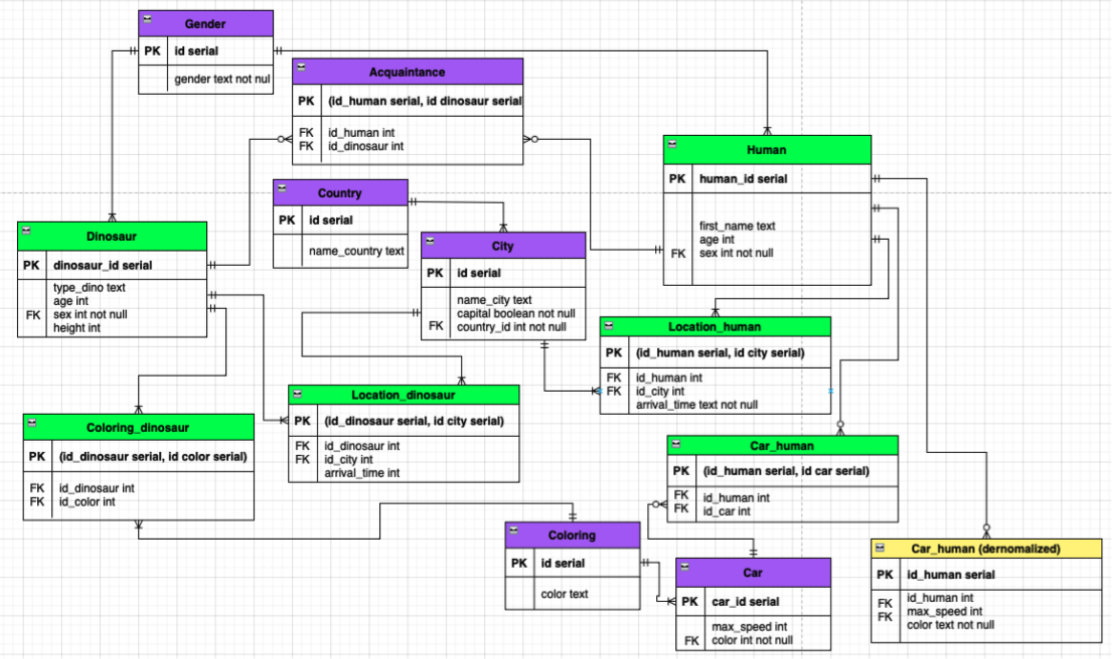
\includegraphics[width=.9\textwidth]{123}